\chapter{Entwurf}
\label{cha:entwurf}

In diesem Kapitel wird der Entwurf der in Kapitel \ref{cha:implementierung} beschriebenen Implementierung erkl"art. In Abschnitt \ref{sec:mep} werden die Message Exchange Pattern definiert und anschlie"send n"aher beschrieben. 

Diese Patterns liefern die Basis f"ur den im Abschnitt \ref{sec:architektur} dargestellten Architekturentwurf der Bibliothek und f"ur das in Abschnitt \ref{sec:protokoll} spezifizierte Protokoll.

\section{Message Exchange Pattern}
\label{sec:mep}

\nomenclature{MEP}{Message Exchange Pattern}

Message Exchange Pattern (MEP) ist eine Bezeichnung f"ur ein Kommunikationsmodell, welches den Austausch von Nachrichten spezifiziert. Aufgrund dieser Patterns kann ein Protokoll, also eine Vereinbarung zwischen Knoten definiert werden, welche Typen von Nachrichten ausgetauscht werden.

Im Folgenden werden nun die Message Exchange Pattern, die in dieser Arbeit Verwendung finden, spezifiziert, wobei der Aufbau dabei wie folgt ist:
\paragraph{\{Pattern\}}
\begin{itemize}
\item \{Anfrage-Typ\}: \{Anzahl\} 
\item \{Antwort-Typ\}: \{Anzahl\}
\end{itemize}
Anmerkung: Die in der Definition verwendete Zahl {\it n} entspricht dabei einer unbekannten, aber endlichen Zahl.

Der Anfrage-/Antwort- Typ hat dabei die folgende Bedeutung:
\begin{itemize}
\item {\it Message}: Nachricht mit der Struktur: {\bf adresse}, {\bf inhalt}
\item {\it Confirmation}: Best"atigung mit der Struktur: {\bf adresse}
\item {\it Request}: Anfrage mit der Struktur: {\bf adresse}, {\bf inhalt}
\item{\it Response}: Antwort mit der Struktur: {\bf adresse}, {\bf inhalt}
\end{itemize}

\pagebreak

\subsection{Definition}
\label{subsec:mep-def}

\subsection*{One-way:}

\paragraph{Unicast}
Eine Unicast Nachricht wird an eine Adresse verschickt. Diese Nachricht beinhaltet einen Inhalt. Optional wird {\it eine} Best"atigung zur"uckgeschickt. Dabei enth"alt eine Best"atigung \emph{keinen} Inhalt.
\paragraph{Multicast}
Eine Multicast Nachricht wird an mehrere Adressen verschickt. Alle Nachrichten beinhalten den selben Inhalt. Optional wird {\it jeweils eine} Best"atigung zur"uckgeschickt. Dabei enthalten die Best"atigungen \emph{keinen} Inhalt. Eine Multicast Nachricht wird erst zum letzt m"oglichen Verteiler vervielf"altigt, entspricht also \emph{nicht} n Unicast Nachrichten.

\begin{figure}[htbp]
\fbox{
\begin{minipage}[t]{0.43\textwidth}
	
\paragraph{Unicast}
\begin{itemize}
\item Message: 1 
\item Confirmation (optional): 1
\end{itemize}

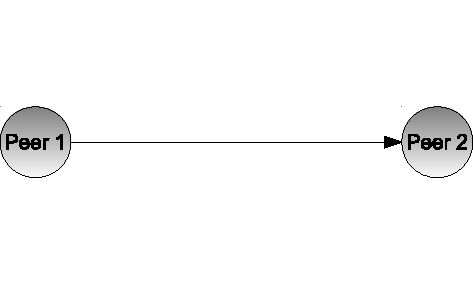
\includegraphics[width=\textwidth]{img/mep_arch_unicast.pdf}
\caption{Unicast}
\label{fig:mep_arch_unicast} 
\end{minipage}
}
\hfill
\fbox{
\begin{minipage}[t]{0.43\textwidth}

\paragraph{Multicast}
\begin{itemize}
\item Message: n  
\item Confirmation (optional): n
\end{itemize}

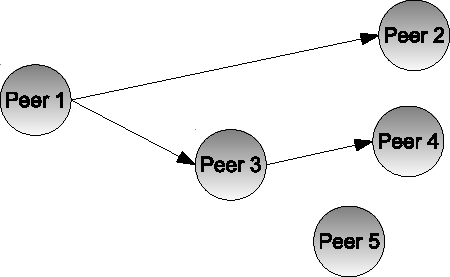
\includegraphics[width=\textwidth]{img/mep_arch_multicast.pdf}
\caption{Multicast}
\label{fig:mep_arch_multicast} 
\end{minipage}
}
\end{figure}

%\subsection*{One-way:}
%\paragraph{Unicast}
%\begin{itemize}
%\item Request: 1 
%\item Confirmation (optional): 1
%\end{itemize}
%\myfig[8 cm]{mep_arch_unicast}{Unicast}
%
%
%
%\paragraph{Multicast}
%\begin{itemize}
%\item Request: n  
%\item Confirmation (optional): n
%\end{itemize}
%\myfig[8 cm]{mep_arch_multicast}{Multicast}
%
%\pagebreak

%\pagebreak

\subsection*{Request-Response:}

%\subsection*{Request-Response:}
%\paragraph{SingleRequestSingleResponse}
%\begin{itemize}
%\item Request: 1  
%\item Response: 1
%\end{itemize}
%\myfig[8 cm]{mep_arch_srsr}{SingleRequestSingleResponse}
%
%\paragraph{SingleRequestMultiResponse}
%\begin{itemize}
%\item Request: 1  
%\item Response: n
%\end{itemize}
%\myfig[8 cm]{mep_arch_srmr}{SingleRequestMultiResponse}

\paragraph{Single Request Single Response}
Eine Single Request Single Response Nachricht entspricht einer Unicast Nachricht, die {\it eine} Antwort zur"uckgeschickt. Diese Antwort enth"alt ebenfalls einen Inhalt.
\paragraph{Single Request Multi Response}
Eine SingleRequestMultiResponse Nachricht entspricht einer Unicast Nachricht, die {\it mehrere} Antworten zur"uckgeschickt. Diese Antworten enthalten ebenfalls jeweils einen Inhalt.
\paragraph{Multi Request Multi Response}
Eine MultiRequestMultiResponse Nachricht entspricht einer Multicast Nachricht, die {\it jeweils eine oder mehrere} Antworten zur"uckgeschickt. Diese Antworten enthalten ebenfalls jeweils einen Inhalt.

\clearpage

\begin{figure}[htbp]
\fbox{
\begin{minipage}[t]{0.43\textwidth}
	
\paragraph{Single Request Single Response}
\begin{itemize}
\item Request: 1 
\item Response: 1
\end{itemize}


\includegraphics[width=\textwidth]{img/mep_arch_srsr.pdf}
\caption{Single Request $ $ $ $ $ $ $ $ Single Response}
\label{fig:mep_arch_srsr} 
\end{minipage}
}
\hfill
\fbox{

\begin{minipage}[t]{0.43\textwidth}
\paragraph{Single Request Multi Response}
\begin{itemize}
\item Request: 1  
\item Response: 1..n
\end{itemize}


\includegraphics[width=\textwidth]{img/mep_arch_srmr.pdf}
\caption{Single Request $ $ $ $ $ $ $ $ $ $ Multi Response}
\label{fig:mep_arch_srmr} 
\end{minipage}
}
\end{figure}

\begin{figure}[!h]
\begin{center}
\fbox{
	\begin{minipage}[t]{0.42\textwidth}
	
\paragraph{Multi Request Multi Response}
\begin{itemize}
\item Request: 1..n 
\item Response: 1..m
\end{itemize}

	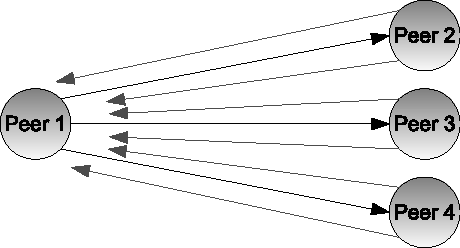
\includegraphics[width=\textwidth]{img/mep_arch_mrmr.pdf}
	\caption{Multi Request $ $ $ $ $ $ $ $ Multi Response}
	\label{fig:mep_arch_mrmr} 
	\end{minipage}
	}
	\end{center}
\end{figure}

%\paragraph{MultiRequestMultiResponse}
%\begin{itemize}
%\item Request: n  
%\item Response: n
%\end{itemize}
%\myfig[8 cm]{mep_arch_mrmr}{MultiRequestMultiResponse}



Aus der oben beschriebenen Definition kann nun, mittels der Unterscheidung zwischen {\it Unreliable} (Anfrage ohne Best"atigung bzw. Antwort) und {\it Reliable} (Anfrage mit Best"atigung bzw. Antwort), das folgende komplette Pattern abgleitet werden:

\begin{itemize}
\item Unreliable Messaging
\begin{itemize}
\item Unreliable Unicast
\item Unreliable Multicast
\end{itemize}
\item Reliable Messaging
\begin{itemize}
\item Reliable Unicast
\item Reliable Multicast
\item Single Request Single Response
\item Single Request Multi Response
\item Multi Request Multi Response
\end{itemize}
\end{itemize}

\subsubsection{Anmerkung}
Bei der Betrachtung der oben beschriebenen Definition k"onnte nun die Frage aufkommen, warum hier zwischen dem {\it Unreliable} und {\it Reliable} Messaging (z.B. bei Unicast-Nachrichten) unterschieden wird. Bei jedem Nachrichtenversand eines Reliable Messaging Pattern wird jeweils eine Best"atigung bzw. Antwort zum Sender zur"uckgeschickt. Dieses bedeutet allerdings sowohl einen zus"atzlichen Netzwerkverkehr als auch eine zus"atzliche Wartezeit auf die Antwort, obwohl diese gegebenfalls gar nicht ben"otigt wird.

\section{Architektur}
\label{sec:architektur}
Wie bereits erw"ahnt setzt diese Bachelorarbeit auf dem Netty-Framework (Abschnitt \ref{sec:netty}) auf. Dementsprechend orientiert sich die gew"ahlte Architektur an diesem Framework. Die Architektur setzt sich dabei aus der Channel-Architektur und der Pipeline-Architektur zusammen.

\subsection{Aufbau}
\label{subsec:mep-arch-channel}

Die gew"ahlte Channel-Architektur ist aus den folgenden Komponenten zusammengesetzt:

\begin{itemize}
\item {\bf Unicast / Multicast Channel}: wird einzig zum Versenden von Unicast und Multicast Nachrichten verwendet.
\item {\bf Single Request Single Response Channel}: wird einzig zum Versenden von Single Request Single Response Nachrichten verwendet.
\item {\bf Multi Response Channel}: wird einzig zum Versenden von Multi Response Nachrichten, namentlich Single Request Multi Response und Multi Request Multi Response verwendet.
\item {\bf RPC Channel}: wird einzig zum Aufruf von Remote Procedure Calls verwendet.
\end{itemize}

\myfig{mep-channel-arch}{Vereinfachte Channel-Architektur}

Die Zusammensetzung der einzelnen Komponenten ist in Abbildung \ref{fig:mep-channel-arch} veranschaulicht, dabei ist die Transportschicht durch das Uberlay-Projekt (Abschnitt \ref{sec:uberlay}) gegeben. Die Channel sind mittels einer Multiplexer / Demultiplexer -Logik, mit der Transportschicht verbunden. Jeder Channel besitzt eine eigene Pipeline, die wiederum Handler enth"alt, die f"ur die Verarbeitung der Nachrichten sorgen. 

\subsection{Erl"auterung}
Die gew"ahlte Architektur, welche oben beschrieben ist,orientiert sich an dem Aufbau der Netty-Architektur. Unicast bzw. Multicast Nachrichten liefern Confirmations zur"uck, die keinen Payload enthalten. Responses des Request-Response-Pattern, namentlich Single Request Single Response, Single Request Multi Response und Multi Request Multi Response liefern Responses zur"uck, welche "uber eigene ChannelFuture-Objekte zur"uckgeliefert werden. Der RPC Channel wiederum erm"oglicht die Benutzung von Protobuf (Abschnitt \ref{sec:google-protobuf}).

%\subsection{Pipeline-Architektur}
%\label{subsec:mep-arch-pipeline}
%Jeder Peer besitzt einen Socket, welcher wie bereits in Kapitel \ref{sec:netty} beschrieben, eine Pipeline, namentlich {\bf ChannelPipeline} enth"alt. Desweiteren enth"alt jeder Peer zus"atzlich noch eine {\bf SingleRequestSingleResponseChannelPipeline} sowie eine {\bf MultiResponseChannelPipeline}. Die Abbildung \ref{fig:mep_arch} zeigt dabei die daraus resultierende Ubermep-Architektur inklusive der Anbindung an das Uberlay-Modul. 
%
%%\myfig[10 cm]{mep_arch}{Ubermep-Pipeline-Architektur mit Anbindung an Uberlay}
%
%Zentraler Einstiegspunkt der Ubermep-Architektur ist der {\bf Peer} welche die {\bf ApplicationChannelPipeline} bereith"alt. Desweiteren verbindet der {\bf Peer} die ApplicationChannelPipeline mit der {\bf SingleRequestSingleResponseChannelPipeline} sowie der {\bf MultiResponseChannelPipeline}. 
%
%Die verschiedenen ChannelPipelines sind dabei wie folgt aufgebaut:
%
%\subsubsection{ApplicationChannelPipeline}
%
%%\myfig[6 cm] {mep-channel-pipeline-arch-a}{Aufbau der ApplicationChannelPipeline}
%
%Die ApplicationChannelPipeline wird dem Uberlay-Module "ubergeben (siehe \ref{sec:uberlay}). Die Handler bzw. Enkoder und Dekoder besitzen dabei die folgenden Aufgaben (von unten nach oben):
%\begin{itemize}
%\item Auf der untersten Ebene befinden sich der {\bf ProtobufEncoder} und {\bf ProtobufDecoder} zum verarbeiten der serialisierten Protobuf-Protokoll-Nachrichten. 
%\item Dar"uber befindet sich der {\bf UnreliableServiceHandler}, verantworlich f"ur die Unreliable Unicast bzw. Unreliable Multicast Nachrichten. 
%\item Dar"uber verarbeitet der {\bf ReliableServiceHandler} die Reliable Nachrichten namentlich Reliable Unicast bzw. Reliable Multicast. Desweiteren besitzt der ReliableServiceHandler den Einstiegspunkt zum Versenden von SingleRequestSingleResponse, SingleRequestMultiResponse und MultiRequestMultiResponse Nachrichten. Diese werden dann an die jeweils zust"andige Pipeline weitergeleitet.
%\item Dar"uber befinden sich s"amtliche manuell am jeweiligen Peer zus"atzlich hinzugef"ugten ServiceHandler (in der Abbildung als AdditionalServiceHandler gekennzeichnet).   Der Benutzer wiederum bestimmt dabei selber die Reihenfolge bei mehrfach hinzugef"ugten ServiceHandlern. 
%\item Ganz oben in der Pipeline befindet sich dann der {\bf RpcServiceHandler} der sich f"ur die Remote Procedure Calls verantworlich zeichnet.
%\end{itemize}
%
%Die nun folgenden Request-Response-Pattern (s. Abschnitt \ref{sec:architektur}) zugeh"origen Pipelines und deren Handler sorgen beim Senden f"ur die Umwandlung in serialisierbare Protokoll-Nachrichten bzw. beim Empfangen f"ur die Umwandlung der serialisierten Protokoll-Nachrichten in ein Objekt des entsprechenden Nachrichtentyps des Message Exchange Patterns.
%
%\subsubsection{SingleRequestSingleResponseChannelPipeline}
%
%%\myfig[9 cm]{mep-channel-pipeline-arch-b}{Aufbau der SingleRequestSingleResponseChannelPipeline}
%
%In der SingleRequestSingelResponsePipeline werden ausschlie"slich die Single\-Request\-Single\-Response-Nachrichten verarbeitet. Sie besitzt nur einen Handler mit der folgenden Aufgabe:
%\begin{itemize}
%\item Der {\bf SingleRequestSingleResponseServiceHandler} verarbeitet den Versand und Empfang von SingleRequestSingleResponse-Nachrichten. 
%\end{itemize}
%
%\subsubsection{MultiResponseChannelPipeline}
%
%%\myfig[7 cm]{mep-channel-pipeline-arch-c}{Aufbau der MultiResponseChannelPipeline}
%
%In der MultiResponseChannelPipeline werden ausschlie"slich die MultiResponse-Nachrichten, namentlich SingleRequestMultiResponse bzw. MultiRequestMultiResponse verarbeitet. Sie besitzt zwei Handler mit den folgenden Aufgaben:
%\begin{itemize}
%\item Auf der untersten Ebene befindet sich der {\bf SingleRequestMultiResponseServiceHandler}, der den Versand und Empfang von Single\-Request\-Multi\-Response-Nachrichten verarbeitet.
%\item Dar"uber befindet sich der {\bf MultiRequestMultiResponseServiceHandler}, der den Versand und Empfang von MultiRequestMultiResponse-Nachrichten verarbeitet.
%\end{itemize}
%
%\subsection{Ubermep-Architektur}
%Der nun folgende Abschnitt beschreibt das Zusammenspiel zwischen der in Abschnitt \ref{subsec:mep-arch-channel} beschriebenen Channel-Architektur und der in Abschnitt \ref{subsec:mep-arch-pipeline} beschriebenen Pipeline-Architektur.
%
%\subsubsection{ApplicationChannel und ApplicationChannelPipeline}
%Die ApplicationChannelPipeline wird nun auf den ApplicationChannel aufgesetzt welcher zwischen dem Sender-Socket und Empf"anger-Socket aufgebaut wird. Die Anbindung der ApplicationChannelPipeline an den ApplicationChannel ist in Abbildung \ref{fig:mep-app_channel-arch} verdeutlicht. Die Abbildung soll dabei das Senden einer Nachricht des {\it One-way} -Pattern veranschaulichen. Die rechte Seite der ApplicationPipeline entspricht der ApplicationPipeline Sender-seitig, die linke Seite der ApplicationPipeline Empf"anger-seitig. Anmerkung: In der Abbildung \ref{fig:mep-app_channel-arch} sind einige ServiceHandler der ApplicationPipeline weggelassen worden, um das Schaubild nicht "ubersichtlich zu halten. Die ApplicationPipeline eines Peers, entspricht {\it immer} der, in Abschnitt \ref{subsec:mep-arch-pipeline} beschriebenen Form. 
%
%Der Ablauf beim Versenden einer One-way-Pattern-Nachricht ist nun wie folgt:
%\begin{itemize}
%\item Am Client (Peer 1) wird das Nachrichten-Objekt des One-way Pattern downstream in der ApplicationChannelPipeline weitergereicht bis der entsprechende ServiceHandler die Nachricht in eine Protokoll-Nachricht umwandelt. 
%\item Diese wird dann mittels des ProtobufEncoder serialisiert
%\item und "uber den ApplicationChannel an den Server (Peer 2) gesendet.
%\item Dort wird dann die serialisierte Nachricht mittels des ProtobufDecoder in eine Protokoll-Nachricht deserialisiert 
%\item und upstream an den entsprechenden ServiceHandler weitergereicht.
%\item Der ServiceHandler wandelt diese Nachricht dann in das entsprechende Nachrichten-Objekt um.
%\end{itemize}
%
%\myfig{mep-app_channel-arch}{Vereinfachte ApplicationChannel und -Pipeline Architektur}
%
%\subsubsection{SingleRequestSingleResponseChannel und SingleRequestSingleResponseChannelPipeline}
%Wie bereits in Abschnitt \ref{subsec:mep-arch-channel} beschrieben ist der SingleRequestSingleResponseChannel mittels einer Multiplexer / Demultiplexer -Logik mit dem ApplicationChannel verbunden. Zus"atzlich ist der SingleRequestSingleResponseChannel Client-seitig sowie Server-seitig mit einer SingleRequestSingleResponseChannelPipeline verbunden. Im folgenden soll nun anhand des Versenden bzw. Empfangen einer SingleRequestSingleResponse-Nachricht das Zusammenspiel der verschiedenen Channels sowie Pipelines verdeutlicht werden. Die Abbildung \ref{fig:mep-srsr_channel-arch} veranschaulicht dabei diesen Ablauf.
%
%\myfig{mep-srsr_channel-arch}{Vereinfachte SingleRequestSingleResponse-Ubermep Architektur}
%
%\begin{itemize}
%\item (1) Der SingleRequestSingleResponseChannel hat beim Versenden einer Single\-Request\-SingleResponse-Nachricht seinen Einstiegspunkt im {\bf ReliableServiceHandler}. 
%\item (2) Dieser (ReliableServiceHandler) leitet diese dann an den SingleRequestSingleResponseChannel weiter und 
%\item (3) der zugeh"orige SingleRequestSingleResponseServiceHandler baut diese Nachricht in eine Protokoll-Nachricht (siehe Abschnitt \ref{sec:protokoll}) um. 
%\item (4) Die ChannelSink leitet diese Protokoll-Nachricht 
%\item (5) dann an den ApplicationChannel weiter. 
%\item (6) Diese wird dann vom ProtobufEncoder encodiert und an den Remote-Peer gesendet. 
%\item (7) Der ReliableServiceHandler des Remote-Hosts bekommt dann diese Nachricht hochgereicht. 
%\item (8) Der SingleRequestSingleResponseServiceHandler empf"angt dann den Protokoll-Nachricht-Request, baut daraus eine Protokoll-Response-Nachricht und 
%\item gibt diese zur"uck and den ReliableServiceHandler. Dieser sendet dann diese Protokoll-Response-Nachricht downstream zur"uck zum Sender. 
%\item Der Sender empf"angt diese Response upstream im ReliableServiceHandler 
%\item und leitet diese an den SingleRequestSingleResponseChannel weiter, 
%\item so dass diese Protokoll-Nachricht im SingleRequestSingleResponseServiceHandler in eine SingleRequestSingle\-Response-Response umgewandelt werden kann. 
%\item Diese wird dann an den ReliableServiceHandler des Senders zur"uckgegeben.
%\end{itemize}
%
%\subsubsection{MultiResponseChannel und MultiResponseChannelPipeline}
%So wie der SingleRequestSingleResponseChannel, ist auch der MultiResponseChannel, wie bereits in Abschnitt \ref{subsec:mep-arch-channel} beschrieben, mittels einer Multiplexer / Demultiplexer -Logik mit dem ApplicationChannel verbunden. Der Ablauf einer MultiResponse-Nachricht, ist dabei analog zu der einer Single\-Request\-Single\-Response-Nachricht. Im folgenden soll deshalb nur auf die Unterschiede eingangen werden, wobei die Abbildung \ref{fig:mep-mr_channel-arch} auch hierbei den Ablauf veranschaulicht:
%
%\begin{itemize}
%\item der ReliableServiceHandler leitet die Nachricht an den MultiResponseChannel weiter
%\item der MultiRequestMultiResponseChannel baut, beim Versand, die Multi\-Request\-Multi\-Response-Nachricht in eine entsprechende Protokoll-Nachricht um
%\item der SingleRequestMultiResponseChannel baut, beim Versand, die Single\-Request\-Multi\-Response-Nachricht in eine entsprechende Protokoll-Nachricht um
%\item der Empfang einer Protokoll-Nachricht im ReliableServiceHandler ist dabei analog zu der oben beschrieben Logik
%\end{itemize}
%
%\myfig{mep-mr_channel-arch}{Vereinfachte MultiResponse-Ubermep Architektur}
%
%\subsubsection{UbermepRpcChannel und ApplicationChannelPipeline}
%Wie bereits im Kapitel \ref{sec:google-protobuf} erw"ahnt setzt die genutzte {\it Remote Procedure Call} -Architektur auf Google Protobuf auf, d.h. der RPC-Channel hat nichts mit den bisherigen beschriebenen (Netty) -Channels gemein, besitzt dementsprechend auch keine entsprechende ChannelPipeline. Trotzdem hat der UbermepRpcChannel einen korrespondierenden ServiceHandler, namentlich {\it RpcServiceHandler}, welcher in der ApplicationChannelPipeline sitzt (siehe Abschnitt \ref{subsec:mep-arch-pipeline}).
%Das Zusammenspiel des UbermepRpcChannel und der ApplicationChannelPipeline soll nun anhand eines Ablaufs eines Ubermep-Remote-Procedure-Calls mit Hilfe der Abbildung \ref{fig:mep-rpc_channel-arch} veranschaulicht werden. 
%
%\myfig{mep-rpc_channel-arch}{Vereinfachte RPC-Ubermep Architektur}
%
%Der Ablauf eines Remote Procedure Calls ist dabei wie folgt, wobei im folgenden der aufrufende Peer als Client und der ausf"uhrende Peer als Server benannt ist. 
%\begin{itemize}
%\item Zuerst wird der aufzurufende Service am Server-Peer registriert (siehe dazu Abschnitt \ref{sec:rpc}).
%\item Anschlie"send wird ein UbermepRpcChannel zum Server aufgebaut.
%\item (1) F"ur diesen Channel wird ein zugeh"origer Stub generiert.
%\item "Uber diesen Stub wird dann die Methode ausgef"uhrt. 
%\item (2) Dabei wird dann "uber den UbermepRpcChannel der RpcServiceHandler aufgerufen. 
%\item (3) Dieser (RpcServiceHandler) wandelt den RPC in eine Protokoll-Nachricht um und leitet diese an den ApplicationChannel des Uberlay-Moduls weiter. 
%\item (4) Anschlie"send wird die Protokoll-Nachricht downstream an den Server-Peer verschickt. 
%\item (5) Am Server-Peer wird diese dann upstream empfangen 
%\item (6) an den RpcServiceHandler weitergereicht
%\item (7) und anschlie"send im Service ausgef"uhrt. 
%\item (8) Das Ergebnis wird dann an den RpcServiceHandler zur"uckgegeben, 
%\item und anschlie"send am Server in eine Protokoll-Antwort umgebaut, 
%\item die dann wiederum "uber den ApplicationChannel im RpcServiceHandler des aufrufenden Clients landet. 
%\item (9) Die Anwort wird schlu"sendlich "uber den UbermepRpcChannel an die aufrufende Methode zur"uckgegeben.
%\end{itemize}


\section{Protokoll}
\label{sec:protokoll}
Im Folgenden Abschnitt werden nun die, im Abschnitt \ref{sec:mep} spezifizierten Message Exchange Pattern in ein Protokoll umgewandelt. Mittels diesem Protokoll k"onnen dann Nachrichtentypen des Message Exchange Pattern "uber den entsprechenden Channel versendet werden.

\subsection{Struktur}
Dieser Abschnitt zeigt den schematischen Aufbau des verwendeten Protokolls und beschreibt deren ben"otigte und optionale Felder. In Abbildung \ref{fig:mep_protokoll} ist die Struktur des Protokolls zu sehen. Dabei sind die optionalen Felder mit * gekennzeichnet. Diese Felder werden nur "ubertragen, wenn sie ben"otigt werden. 
\myfig{mep_protokoll}{Schematischer Aufbau des Protokolls}

Die in Abbildung \ref{fig:mep_protokoll} beschriebenen Felder haben die folgende Bedeutung: 

\begin{itemize}
\item {\bf ID}: erm"oglicht die eindeutige Identifizierung einer Nachricht.
\item {\bf Typ}: besteht aus einem der folgenden m"oglichen Nachrichtentypen:
\begin{itemize}
\item UNICAST
\item MULTICAST
\item SINGLE\_RESPONSE\_REQUEST
\item MULTI\_RESPONSE\_REQUEST
\item SINGLE\_RESPONSE
\item MULTI\_RESPONSE
\item RPC\_REQUEST
\item RPC\_RESPONSE
\end{itemize}
\item Das Flag {\bf Reliable} wird gesetzt falls eine Nachricht zu dem \emph{Reliable Messaging} Pattern geh"ort.
\item {\bf Akt. Nachricht}: wird \emph{nur} f"ur MultiResponse-Nachrichten "ubertragen. Dieses Feld zeigt an welche Nummer die entsprechende Response besitzt. Beispiel: \emph{(Aktuelle Nachricht)} {\bf 2}, von \emph{(Anzahl Nachrichten)} 4.
\item {\bf Anz. Nachrichten}: wird \emph{nur} f"ur MultiResponse-Nachrichten ben"otigt und beschreibt die zu erwartenden Responses. 
\item {\bf Payload}: enth"alt den zu "ubertragenen Inhalt.
\end{itemize}
%\paragraph{ID}
%Die \emph{ID} erm"oglicht die eindeutige Identifizierung einer Nachricht.

%\paragraph{Typ}
%Ein \emph{Typ} besteht aus einem der folgenden m"oglichen Nachrichtentypen:
%\begin{itemize}
%\item UNICAST
%\item MULTICAST
%\item SINGLE\_RESPONSE\_REQUEST
%\item MULTI\_RESPONSE\_REQUEST
%\item SINGLE\_RESPONSE
%\item MULTI\_RESPONSE
%\item RPC\_REQUEST
%\item RPC\_RESPONSE
%\end{itemize}

%\paragraph{Reliable}
%Das Flag \emph{Reliable} wird gesetzt falls eine Nachricht zu dem \emph{Reliable Messaging Pattern} geh"ort.

%\paragraph{Akt. Nachricht}
%Das Feld \emph{Aktuelle Nachricht} wird \emph{nur} f"ur MultiResponse-Nachrichten ben"otigt. Dieses Feld zeigt an welche Nummer die entsprechende Response besitzt. Beispiel: \emph{(Aktuelle Nachricht)} {\bf 2} von \emph{(Anzahl Nachrichten)} 4.

%\paragraph{Anz. Nachrichten}
%Das Feld \emph{Anzahl Nachrichten} beschreibt die zu erwartenden Responses und wird \emph{nur} f"ur MultiResponse-Nachrichten ben"otigt.

%\paragraph{Payload}
%Das Feld \emph{Payload} enth"alt den zu "ubertragenen Inhalt.

\subsection{Nachrichten}
Im Folgenden wird nun die oben spezifizierte Struktur auf die Nachrichtentypen des Message Exchange Pattern angewendet. Dabei wurden in der Beschreibung die Felder \emph{ID} und \emph{Payload} nicht ber"ucksichtigt, da diese auf die, in diesem Entwurf dargestellten, unterschiedlichen Nachrichtentypen keinen Einfluss haben. Des weiteren werden die Elemente \emph{x} und \emph{-} eingef"uhrt. Sie besitzen die folgende Bedeutung:

\begin{tabular}{rl}
x & := gesetzt \\
- & := nicht gesetzt \\
 \end{tabular}

\begin{figure}[h]
\subsubsection{Unreliable Messaging}

\subsubsection{\hspace{10mm} Unreliable Unicast}
\subfigure[Unreliable Unicast-Request]{
\label{fig:mep_protokoll_unrel_unicast}
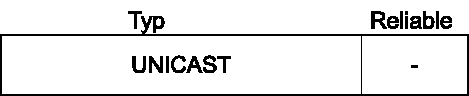
\includegraphics{img/mep_protokoll_unrel_unicast.pdf}
%\caption{UnreliableUnicast-Request}
}

\subsubsection{\hspace{10mm} Unreliable Multicast}
\subfigure[Unreliable Multicast-Request]{
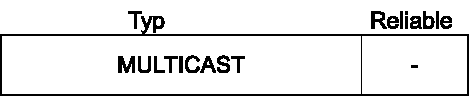
\includegraphics{img/mep_protokoll_unrel_multicast.pdf}
\label{fig:mep_protokoll_unrel_multicast} 
}
\end{figure}

\begin{figure}[h]
\subsubsection{Reliable Messaging}

\subsubsection{\hspace{10mm} Reliable Unicast}
\subfigure[Reliable Unicast-Request]{
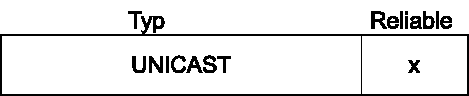
\includegraphics{img/mep_protokoll_rel_unicast.pdf}
\label{fig:mep_protokoll_rel_unicast} 
}

\subsubsection{\hspace{10mm} Reliable Multicast}
\subfigure[Reliable Multicast-Request]{
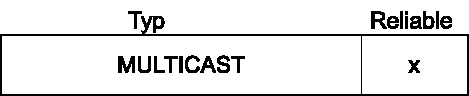
\includegraphics{img/mep_protokoll_rel_multicast.pdf}
\label{fig:mep_protokoll_rel_multicast}
}
\end{figure}

\begin{figure}[h]
\subsubsection{\hspace{10mm} Single Request Single Response}
\subfigure[Single Request Single Response-Request]{
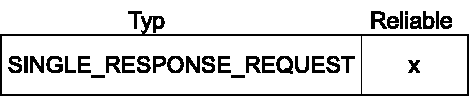
\includegraphics{img/mep_protokoll_srsr_req.pdf}
\label{fig:mep_protokoll_srsr_req} 
}

\subfigure[Single Request Single Response-Response]{
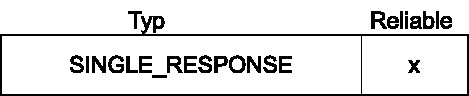
\includegraphics{img/mep_protokoll_srsr_res.pdf}
\label{fig:mep_protokoll_srsr_res}  
}
\end{figure}

\clearpage

\begin{figure}[h]
\subsubsection{\hspace{10mm} Multi Response}
Im Folgenden werden Single Request Multi Response und Multi Request Multi Response Nachrichten in einem \emph{Multi Response}-Typ zusammengefasst.
Die Unterscheidung hierbei wird "uber das Feld ID geregelt.
\subfigure[Multi Response-Request]{
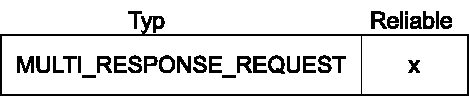
\includegraphics{img/mep_protokoll_mr_req.pdf}
\label{fig:mep_protokoll_mr_req} 
}

\subfigure[Multi Response-Response]{
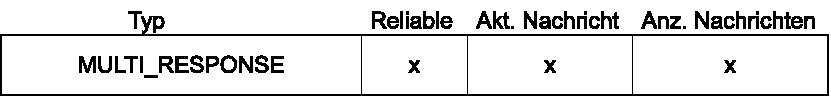
\includegraphics{img/mep_protokoll_mr_res.pdf}
\label{fig:mep_protokoll_mr_res}  
}
\end{figure}

\begin{figure}[h]
\subsubsection{Remote Procedure Call}
\subfigure[RPC-Request]{
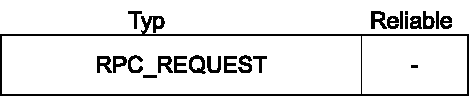
\includegraphics{img/mep_protokoll_rpc_req.pdf}
\label{fig:mep_protokoll_rpc_req} 
}

\subfigure[RPC-Response]{
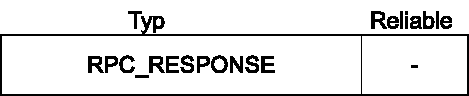
\includegraphics{img/mep_protokoll_rpc_res.pdf}
\label{fig:mep_protokoll_rpc_res}  
}
\end{figure}
